\section{Experimental Results}

\subsection{Simulated Runs}
We simulated performance of our algorithms on random graphs generated
by the graph models we outlined. 
%Arda: We mention fixed degree and Erdos-Renyi above - which one are you talking about here in the experiments?
In the following figures, each data
point is obtained by averaging the measurements over 10 random
graphs. We first present the time and space usage of these algorithms when
solving a $(3,3)$-recommendation subgraph problem in different sized graphs.
Note that varying the value of $a$ and $c$ would only change space and time
usage by a constant, so these two graphs are indicative of time and space
usage over all ranges of parameters

\begin{figure}[t]
\centering
\begin{minipage}[h]{0.48\textwidth}
\centering
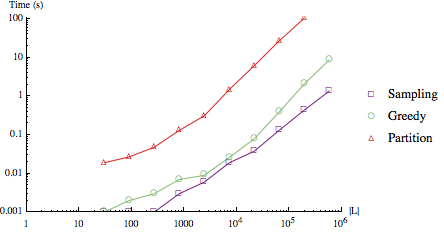
\includegraphics[width=0.8\textwidth]{images/time.png}
\caption{Time needed to solve a (3,3)-recommendation problem in random graphs where $|R|/|L|=4$ (Notice the log-log scale.)}\label{fig:time_graph}
\end{minipage}
\hspace{0cm}
\begin{minipage}[h]{0.48\textwidth}
\centering
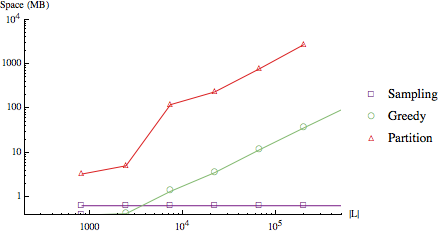
\includegraphics[width=0.8\textwidth]{images/space.png}
\caption{Space needed to solve a (3,3)-recommendation problem in random graphs where $|R|/|L|=4$ (Notice the log-log scale.)}\label{fig:space_graph}
\end{minipage}
\vspace{-0.2in}
\end{figure}
\vs

Recall that the partition algorithm split the graph into multiple graphs
and found matchings in these smaller graphs which were then combined into
a recommendation subgraph. For this reason, a run of the partition
algorithm takes much longer to solve a problem instance than either the
sampling or greedy algorithms. It also takes significantly more memory to
run. This can easily be seen in Figure~\ref{fig:time_graph} and Figure~\ref{fig:space_graph}.
%Arda: What is the relation of the size of R to that of L in these figures? Say it in the captions!!
%Arda: In both these figures, change the annotation of three algorithms to the corresponding type of point in the series (triangle, circle etc.) as in the later figures.
Compare this to greedy and sampling which both require a single pass over
the graph, and no advanced data structures. In fact, if the adjacency list
of $G$ is pre-sorted by the edge's endpoint in $L$, then the sampling algorithm can be
implemented as an online algorithm with constant space and in constant time 
per link selection. Similarly, if the adjacency list of $G$
is pre-sorted by the edge's endpoint in $R$, then the greedy algorithm can
be implemented so that the entire graph does not have to be kept in memory. In this
event, greedy uses only $O(|L|)$ memory.\vs

Next, we analyze the relative qualities of the solutions each method
produces.  Figures~\ref{fig:a=1:1} and \ref{fig:a=1:2} plot the
average performance ratio of the three methods compared to the trivial
upper bounds as the value of $c$, the number of recommendations
allowed is varied, while keeping $a = 1$.
%Arda: First say what these figures are depicting, i.e., what is the y-axis and the x-axis
They collectively show that the lower bound we calculated for the
expected performance of the sampling algorithm accurately captures the
behavior of the sampling algorithm when $a=1$. Indeed, the inequality
we used is an accurate approximation of the expectation, up to lower
order terms, as is demonstrated in these simulated runs.  The random
sampling algorithm does well, both when $c$ is low and high, but
falters when $ck=1$. The greedy algorithm performs better than the
random sampling algorithm in all cases, but its advantage vanishes as
$c$ gets larger. Note that the dip in the graphs when $cl=ar$, at
$c=4$ in Figure~\ref{fig:a=1:1} and $c=2$ in Figure~\ref{fig:a=1:2} is
expected and was previously demonstrated in
Figure~\ref{fig:simple_approx}.  The partition algorithm is immune to
this drop that affects both the greedy and the sampling algorithms,
but comes with the cost of higher time and space utilization.

\begin{figure}[t]
\centering
\begin{minipage}[h]{0.48\textwidth}
\centering
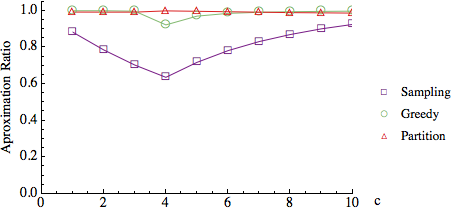
\includegraphics[width=0.8\textwidth]{images/l=25000,r=100000_Greedy_vs_Naive.png}
\caption{$|L|=25$k, $|R|=100$k, $d=20$, $a=1$}\label{fig:a=1:1}
\end{minipage}
\hspace{0cm}
\begin{minipage}[h]{0.48\textwidth}
\centering
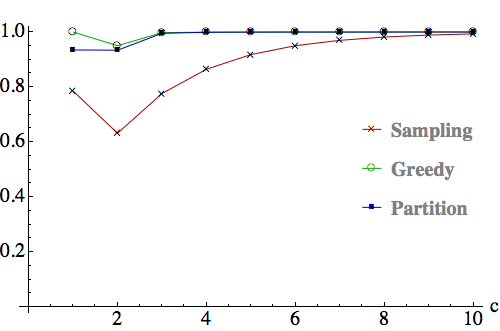
\includegraphics[width=0.8\textwidth]{images/l=50000,r=100000_Greedy_vs_Naive.png}
\caption{$|L|=50$k, $|R|=100$k, $d=20$, $a=1$}\label{fig:a=1:2}
\end{minipage}
\vspace{-0.2in}
\end{figure}


\vs In contrast to the case when $a=1$, the sampling algorithm
performs worse when $a>1$ but performs increasingly better with $c$ as
demonstrated by Figures~\ref{fig:a=2} and \ref{fig:a=4}. The greedy
algorithm continues to produce solutions that are nearly optimal,
regardless of the settings of $c$ and $a$, even winning over the
partition algorithm with increasing values of $a$. Our simulations
suggest that in most cases, one can simply use the very simple
sampling method for solving the $(c, a)$-recommendation subgraph
problem. In those cases where the sampling is not suitable as flagged
by our analysis, we still find that the greedy performs adequately and
is also simple to implement. These two algorithms thus confirm to our
requirements we initially laid out for deployment in large-scale real
systems in practice.


\begin{figure}[t]
\centering
\begin{minipage}[h]{0.48\textwidth}
\centering
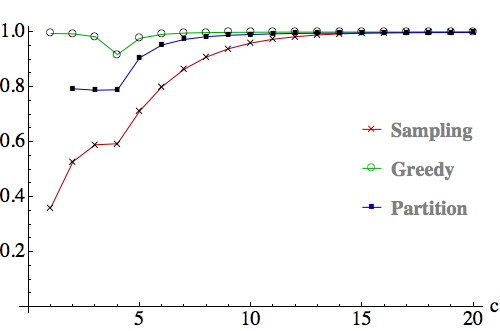
\includegraphics[width=0.8\textwidth]{images/l=50000,r=100000,a=2_Greedy_vs_Naive.png}
\caption{$|L|=50$k, $|R|=100$k, $d=20$, $a=2$}\label{fig:a=2}
\end{minipage}
\hspace{0cm}
\begin{minipage}[h]{0.48\textwidth}
\centering
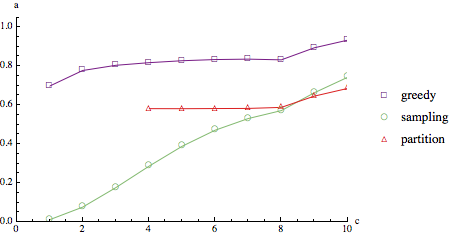
\includegraphics[width=0.8\textwidth]{images/l=50000,r=100000,a=4_Greedy_vs_Naive.png}
\caption{$|L|=50$k, $|R|=100$k, $d=20$, $a=4$}\label{fig:a=4}
\end{minipage}
\vspace{-0.2in}
\end{figure}

\vs
To summarize, our synthetic experiments show the following strengths of each algorithm:\\

\textbf{Sampling Algorithm:} This algorithm uses little to no memory and can
be implemented as an online algorithm. If keeping the underlying graph in
memory is an issue, then chances are this algorithm will do well while only needing
a fraction of the resources the other two algorithms would need.\\

\textbf{Partition Algorithm:} This algorithm does well, but only when $a$ is small.
In particular, when $a=1$ or 2, partition seems to be the best algorithm, but the quality
of the solutions degrade quickly after that point. However this performance comes at
expense of significant runtime and space. Since greedy performs almost as well without
requiring large amounts of space or time, partition is best suited for instances where
$a$ is low the quality of the solution is more important than anything else.\\

\textbf{Greedy Algorithm:} This algorithm is the all-round best performing algorithm we tested.
It only requires a single pass over the data thus running very quickly,  and uses
relatively little amounts of space enabling it run completely in memory for graphs with
as many as tens of millions of edges. It is not as fast as sampling or accurate as partition
when $a$ is small, but it has very good performance over all parameter ranges. 
